% questions.tex —— 2006 年·普通高等学校招生考试·湖南卷文科 · 题目内容片段（无答案）
% 由 tools/generate_projects.py 依来源总账自 2006/2006_数学真题_湖南文_试题.md 生成，勿手改（改源 MD 后重跑）


\begin{gktip}
\textbf{来源及状态}：据本机固定 PDF 第 1–2 页逐题目视转录；文件 SHA-256 与 source manifest 中固定候选副本记录一致。首页题签为“2006 普通高等学校招生考试（湖南卷文）”。题签和字节指纹不能认证发布者、版次、来源链或官方原件身份。固定 PDF 未见答案、解析或评分标准，官方答案未录入。

\textbf{源页定位}：PDF 第 1 页（印刷页码 303）含 Q1–Q18；第 2 页（印刷页码 304）含 Q19–Q21。选择题 Q1–Q10，填空题 Q11–Q15，解答题 Q16–Q21。

\textbf{题图}：Q10 为向量区域图，题干在左栏下部、图和选项在右栏上部；Q18 为两个共底正四棱锥的空间几何图。下列图稿据固定源页结构矢量重绘。
\end{gktip}

\gkpart{一、选择题}

\begin{question}
\gkti{1}函数 $y=\sqrt{\log_2 x}$ 的定义域是\mbox{（　　）}

\begin{gkopts}(4)
\task （A）$(0,1]$
\task （B）$(0,+\infty)$
\task （C）$(1,+\infty)$
\task （D）$[1,+\infty)$
\end{gkopts}

\end{question}
\begin{question}
\gkti{2}已知向量 $\vec a=(2,t),\ \vec b=(1,2)$，若 $t=t_1$ 时，$\vec a\parallel\vec b$；$t=t_2$ 时，$\vec a\perp\vec b$，则\mbox{（　　）}

\begin{gkopts}(2)
\task （A）$t_1=-4,\ t_2=-1$
\task （B）$t_1=-4,\ t_2=1$
\task （C）$t_1=4,\ t_2=-1$
\task （D）$t_1=4,\ t_2=1$
\end{gkopts}

\end{question}
\begin{question}
\gkti{3}若 $(ax-1)^5$ 的展开式中 $x^3$ 的系数是 80，则实数 $a$ 的值是\mbox{（　　）}

\begin{gkopts}(4)
\task （A）$-2$
\task （B）$2\sqrt2$
\task （C）$\sqrt[3]{4}$
\task （D）$2$
\end{gkopts}

\end{question}
\begin{question}
\gkti{4}过半径为 2 的球 $O$ 表面上一点 $A$ 作球 $O$ 的截面，若 $OA$ 与该截面所成的角是 $60^\circ$，则该截面的面积是\mbox{（　　）}

\begin{gkopts}(4)
\task （A）$\pi$
\task （B）$2\pi$
\task （C）$3\pi$
\task （D）$2\sqrt3\pi$
\end{gkopts}

\end{question}
\begin{question}
\gkti{5}“$a=1$”是“函数 $f(x)=|x-a|$ 在区间 $[1,+\infty)$ 上为增函数”的\mbox{（　　）}

\begin{gkopts}(2)
\task （A）充分不必要条件
\task （B）必要不充分条件
\task （C）充要条件
\task （D）既不充分也不必要条件
\end{gkopts}

\end{question}
\begin{question}
\gkti{6}在数字 1，2，3 与符号 $+,-$ 五个元素的所有全排列中，任意两个数字都不相邻的全排列个数是\mbox{（　　）}

\begin{gkopts}(4)
\task （A）6
\task （B）12
\task （C）18
\task （D）24
\end{gkopts}

\end{question}
\begin{question}
\gkti{7}圆 $x^2+y^2-4x-4y-10=0$ 上的点到直线 $x+y-14=0$ 的最大距离与最小距离的差是\mbox{（　　）}

\begin{gkopts}(4)
\task （A）36
\task （B）18
\task （C）$6\sqrt2$
\task （D）$5\sqrt2$
\end{gkopts}

\end{question}
\begin{question}
\gkti{8}设点 $P$ 是函数 $f(x)=\sin\omega x$ 的图象 $C$ 的一个对称中心，若点 $P$ 到图象 $C$ 的对称轴上的距离的最小值是 $\dfrac{\pi}{4}$，则 $f(x)$ 的最小正周期是\mbox{（　　）}

\begin{gkopts}(2)
\task （A）$2\pi$
\task （B）$\pi$
\task （C）$\dfrac{\pi}{2}$
\task （D）$\dfrac{\pi}{4}$
\end{gkopts}

\end{question}
\begin{question}
\gkti{9}过双曲线 $M:x^2-\dfrac{y^2}{b^2}=1$ 的左顶点 $A$ 作斜率为 1 的直线 $l$，若 $l$ 与双曲线 $M$ 的两条渐近线分别相交于点 $B,C$，且 $|AB|=|BC|$，则双曲线 $M$ 的离心率是\mbox{（　　）}

\begin{gkopts}(2)
\task （A）$\dfrac{\sqrt5}{2}$
\task （B）$\dfrac{\sqrt{10}}{3}$
\task （C）$\sqrt5$
\task （D）$\sqrt{10}$
\end{gkopts}

\Needspace{0.4\textheight}
\end{question}
\begin{question}
\gkti{10}如图，$OM\parallel AB$，点 $P$ 由射线 $OM$、线段 $OB$ 及 $AB$ 的延长线围成的阴影区域内（不含边界），且 $\overrightarrow{OP}=x\overrightarrow{OA}+y\overrightarrow{OB}$，则实数对 $(x,y)$ 可以是\mbox{（　　）}

\begin{gkopts}(2)
\task （A）$\left(\dfrac14,\dfrac34\right)$
\task （B）$\left(-\dfrac23,\dfrac23\right)$
\task （C）$\left(-\dfrac14,\dfrac34\right)$
\task （D）$\left(-\dfrac15,\dfrac75\right)$
\end{gkopts}
\nopagebreak[4]
\begin{center}% 2006 湖南文科候选卷 Q10；按固定源图的阴影边界重绘，坐标不表示长度比例。
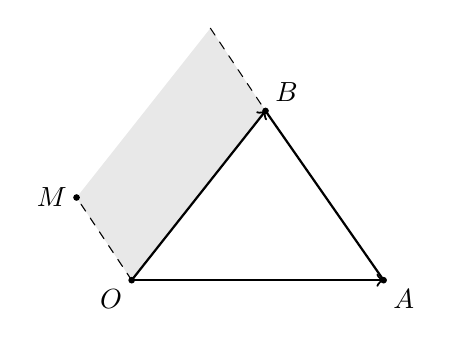
\begin{tikzpicture}[line cap=round,line join=round]
  \coordinate (O) at (0,0);
  \coordinate (A) at (3.2,0);
  \coordinate (B) at (1.7,2.15);
  \coordinate (M) at (-0.7,1.05);
  \coordinate (T) at (1.0,3.2);

  \fill[gray!18] (O)--(M)--(T)--(B)--cycle;

  \draw[dashed] (O)--(M);
  \draw[dashed] (T)--(B);
  \draw[thick] (B)--(A);
  \draw[->,thick] (O)--(B);
  \draw[->,thick] (O)--(A);

  \fill (O) circle[radius=1.2pt];
  \fill (A) circle[radius=1.2pt];
  \fill (B) circle[radius=1.2pt];
  \fill (M) circle[radius=1.2pt];
  \node[below left] at (O) {$O$};
  \node[below right] at (A) {$A$};
  \node[above right] at (B) {$B$};
  \node[left] at (M) {$M$};
\end{tikzpicture}
\end{center}
\nopagebreak[4]
\end{question}
\gkpart{二、填空题}

\begin{question}
\gkti{11}若数列 $\{a_n\}$ 满足：$a_1=1,\ a_{n+1}=2a_n,\ n=1,2,3,\ldots$，则 $a_1+a_2+\cdots+a_n=$ \gkblank{}。

\end{question}
\begin{question}
\gkti{12}某高校有甲、乙两个数学建模兴趣班。其中甲班 40 人，乙班 50 人。现分析两个班的一次考试成绩，算得甲班的平均成绩是 90 分，乙班的平均成绩是 81 分，则该校数学建模兴趣班的平均成绩是 \gkblank{} 分。

\end{question}
\begin{question}
\gkti{13}已知
\nopagebreak[4]
\[
\begin{cases}
x\geqslant1,\\
x-y+1\leqslant0,\\
2x-y-2\leqslant0,
\end{cases}
\]
则 $x^2+y^2$ 的最小值是 \gkblank{}。

\end{question}
\begin{question}
\gkti{14}过三棱柱 $ABC-A_1B_1C_1$ 的任意两条棱的中点作直线，其中与平面 $ABB_1A_1$ 平行的直线共有 \gkblank{} 条。

\end{question}
\begin{question}
\gkti{15}若 $f(x)=a\sin\left(x+\dfrac{\pi}{4}\right)+3\sin\left(x-\dfrac{\pi}{4}\right)$ 是偶函数，则 $a=$ \gkblank{}。

\end{question}
\gkpart{三、解答题}

\begin{question}
\gkti{16}已知
\nopagebreak[4]
\[
\sqrt3\sin\theta-\frac{\sin\left(\frac{\pi}{2}-2\theta\right)}{\cos(\pi+\theta)}\cdot\cos\theta=1,\qquad \theta\in(0,\pi),
\]
求 $\theta$ 的值。

\end{question}
\begin{question}
\gkti{17}某安全生产监督部门对 5 家小型煤矿进行安全检查（简称安检）。若安检不合格，则必须整改。若整改后经复查仍不合格，则强制关闭。设每家煤矿安检是否合格是相互独立的，且每家煤矿整改前安检是合格的概率是 0.5，整改后安检合格的概率是 0.8，计算（结果精确到 0.01）：

（1） 恰好有两家煤矿必须整改的概率；

（2） 某煤矿不被关闭的概率；

（3） 至少关闭一家煤矿的概率。

\Needspace{0.4\textheight}
\end{question}
\begin{question}
\gkti{18}如图，已知两个正四棱锥 $P-ABCD$ 与 $Q-ABCD$ 的高都是 2，$AB=4$。

（1） 证明：$PQ\perp$ 平面 $ABCD$；

（2） 求异面直线 $AQ$ 与 $PB$ 所成的角；

（3） 求点 $P$ 到平面 $QAD$ 的距离。
\nopagebreak[4]
\begin{center}% 2006 湖南文科候选卷 Q18；两个共底正四棱锥，按源图结构重绘，不按比例。
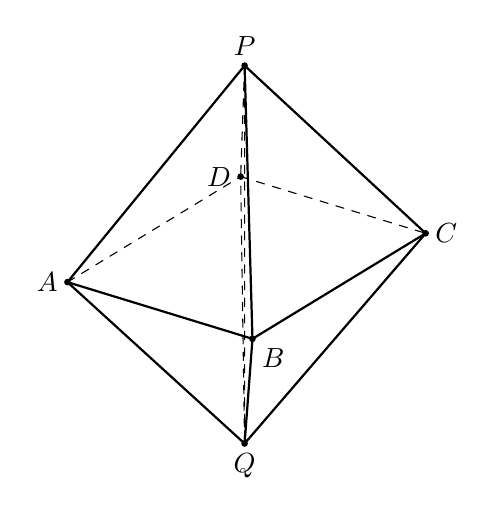
\begin{tikzpicture}[line cap=round,line join=round]
  \coordinate (A) at (-2.2,0);
  \coordinate (B) at (0.15,-0.72);
  \coordinate (C) at (2.35,0.62);
  \coordinate (D) at (0.0,1.34);
  \coordinate (P) at (0.05,2.75);
  \coordinate (Q) at (0.05,-2.05);

  % Hidden back edges and the common altitude line.
  \draw[dashed] (A)--(D) (D)--(C);
  \draw[dashed] (P)--(D) (Q)--(D) (P)--(Q);

  % Visible base and lateral edges.
  \draw[thick] (A)--(B)--(C);
  \draw[thick] (P)--(A) (P)--(B) (P)--(C);
  \draw[thick] (Q)--(A) (Q)--(B) (Q)--(C);

  \foreach \pt in {A,B,C,D,P,Q}{\fill (\pt) circle[radius=1.2pt];}
  \node[left] at (A) {$A$};
  \node[below right] at (B) {$B$};
  \node[right] at (C) {$C$};
  \node[left] at (D) {$D$};
  \node[above] at (P) {$P$};
  \node[below] at (Q) {$Q$};
\end{tikzpicture}
\end{center}
\nopagebreak[4]
\end{question}
\begin{question}
\gkti{19}已知函数 $f(x)=ax^3-3x^2+1-\dfrac3a$。

（1） 讨论函数 $f(x)$ 的单调性；

（2） 若曲线 $y=f(x)$ 上两点 $A,B$ 的切线都与 $y$ 轴垂直，且线段 $AB$ 与 $x$ 轴有公共点，求实数 $a$ 的取值范围。

\end{question}
\begin{question}
\gkti{20}在 $m\ (m\geqslant2)$ 个不同数的排列 $P_1P_2\cdots P_m$ 中，若 $1\leqslant i\leqslant j\leqslant m$ 时 $P_i>P_j$（即前面某数大于后面某数），则称 $P_i$ 与 $P_j$ 构成一个逆序。一个排列的全部逆序的总数称为该排列的逆序数。记排列 $(n+1)n(n-1)\cdots321$ 的逆序数为 $a_n$，如排列 21 的逆序数 $a_1=1$，排列 321 的逆序数 $a_2=3$，排列 4321 的逆序数 $a_3=6$。

（1） 求 $a_4,a_5$，并写出 $a_n$ 的表达式；

（2） 令 $b_n=\dfrac{a_n}{a_{n+1}}+\dfrac{a_{n+1}}{a_n}$，证明：$2n<b_1+b_2+\cdots+b_n<2n+3,\ n=1,2,\ldots$。

\begin{gktip}
Q20 的条件在固定原页中印作 $1\leqslant i\leqslant j\leqslant m$，本稿按原样转录，未据定义或题意改写。
\end{gktip}

\end{question}
\begin{question}
\gkti{21}已知椭圆 $C_1:\dfrac{x^2}{4}+\dfrac{y^2}{3}=1$，抛物线 $C_2:(y-m)^2=2px\ (p>0)$，且 $C_1,C_2$ 的公共弦 $AB$ 过椭圆 $C_1$ 的右焦点。

（1） 当 $AB\perp x$ 轴时，求 $m,p$ 的值，并判断抛物线 $C_2$ 的焦点是否在直线 $AB$ 上；

（2） 若 $p=\dfrac43$ 且抛物线 $C_2$ 的焦点在直线 $AB$ 上，求 $m$ 的值及直线 $AB$ 的方程。

\par\medskip

\begin{gktip}
\textbf{来源说明}：题面据来源总账登记的固定候选 PDF 转录；文件 SHA-256 与 Git blob 见 \texttt{source-manifest.json}，逐题页码和来源指纹见本卷 \texttt{provenance.json}。发布者、版次、来源链及官方身份未核；固定 PDF 不含答案或解析。
\end{gktip}

\end{question}